\documentclass[border=3pt,tikz]{standalone}
\usepackage{amsmath}
\usetikzlibrary{arrows.meta}
\usetikzlibrary{calc}
\begin{document}
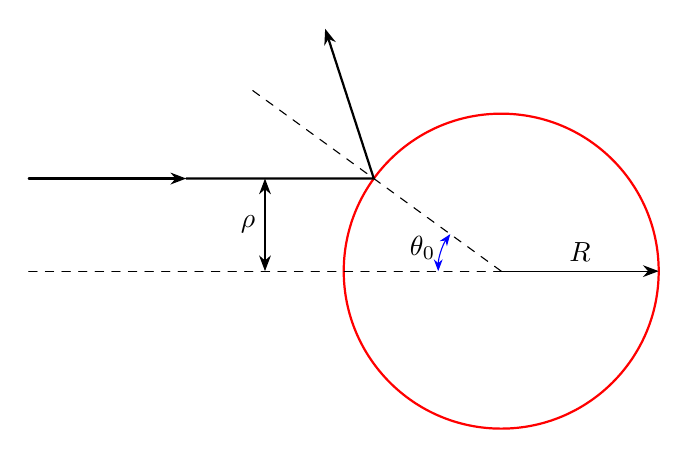
\begin{tikzpicture}[line cap=round, scale = 2]
    \coordinate (A) at (-0.809, 0.588);
    \draw[fill=none, red, thick](0,0) circle (1);
    \draw[dashed] (-3, 0) -- (0, 0);
    \draw[thick, -{Stealth[length=2mm]}] (-3, 0.588) -- (-2, 0.588);
    \draw[thick, -{Stealth[length=2mm]}] (-2, 0.588) -- (A) -- ($(A) + (-0.309, 0.951)$);
    \draw[dashed] (0, 0) -- ($2*(A)$);
    \draw[{Stealth[length=2mm]}-{Stealth[length=2mm]}] (-1.5, 0) -- (-1.5, 0.588);
    \node[left] at (-1.5, 0.295) {$\rho$};
    \draw [blue, {Stealth[length=1.5mm]}-{Stealth[length=1.5mm]}] (-0.4,0.0) arc (180:144:0.4);
    \node [scale=1] at (-0.5, 0.15) {$\theta_0$};
    \draw [-{Stealth[length=2mm]}] (0, 0) -- (1, 0);
    \node [above] at (0.5, 0) {$R$};
    \end{tikzpicture}
\end{document}